% !TEX encoding = UTF-8 Unicode

\documentclass[12pt,oneside]{amsart}
\usepackage{cancel}
\usepackage{xspace}
\usepackage{graphicx}
\usepackage{multicol}
\usepackage{subfig}
\usepackage{amsmath}
\usepackage{amssymb}
\usepackage[a4paper,width=165mm,top=20mm,bottom=25mm,includeheadfoot]{geometry}
\usepackage{array}
\usepackage{verbatim}
\usepackage{caption}
\usepackage{natbib}
\usepackage{float}
\usepackage{pdflscape}
\usepackage{mathtools}
\usepackage[usenames,dvipsnames]{xcolor}
\usepackage{afterpage}
\usepackage{tikz}
\usepackage[bookmarks=true, unicode=true, pdftitle={Nexty Yellow Paper: a formal specification of Nexty, a zero transfer fee and instant transfer base on Ethereum blockchain}, pdfauthor={Thanh Dao / Ha Dang},pdfkeywords={Nexty, Ethereum, Yellow Paper, blockchain, virtual machine, cryptography, decentralised, singleton, transaction, generalised, zero transfer fee, instant transfer},pdfborder={0 0 0.5 [1 3]}]{hyperref}
%,pagebackref=true

\PassOptionsToPackage{hyphens}{url}\usepackage{hyperref}

\makeatletter
 \newcommand{\linkdest}[1]{\Hy@raisedlink{\hypertarget{#1}{}}}
\makeatother
\usepackage{seqsplit}

% For formatting
%\usepackage{underscore}
%\usepackage{lipsum} % to generate filler text for testing of document rendering
\usepackage[english]{babel}
\usepackage[autostyle]{csquotes}
\MakeOuterQuote{"}

\definecolor{pagecolor}{rgb}{1,0.98,0.9}

%Path relative to the main .tex file 
\graphicspath{ {./images/} }

\title{NEXTY: A CONSENSUS TO GET ZERO TRANSFER FEE AND INSTANT TRANSFER BLOCKCHAIN}
\author{
	Thanh Dao \& Ha Dang \\
	Co-founder/CTO @ Nexty Platform \\
	thanhdao@nexty.io / hadang@nexty.io
}
\date{} % delete this line to display the current date

%%% BEGIN DOCUMENT
\begin{document}

\pagecolor{pagecolor}
\begin{abstract}
This is the detail technical paper of \href{https://nexty.io}{Nexty Platform}, focusing on describing the operation of a consensus protocol called Proof of Foundation. Proof of Foundation was inspired by the Proof of Authority introduced by \cite{clique} with improvement from \href{https://nexty.io}{Nexty Platform} by introducing a new confirmation system named \textbf{DCCS} - \textbf{D}ual \textbf{C}ryptocurrency \textbf{C}onfirmation \textbf{S}ystem to achieve a decentralized system and bring a highly incentive system for blockchain maintainers.
\end{abstract}

\maketitle

\setlength{\columnsep}{20pt}
\begin{multicols}{2}
%\tableofcontents

\section{Introduction}\label{sec:introduction}
In addition to {\small NTY} coin-base, {\small DCCS} has the secondary token named {\small NTF}. {\small NTF} is used for authorizing an account to become the maintainer/sealer of the confirmation system described detail in section \ref{sec:authorize}, as well as to calculate reward for block sealer. {\small NTF} token has total supply of $10,000,000$ and will be distributed for the first $100,000,000,000$ NTY holders that joined in ``Smart Staking'' program described detail in the white paper of \cite{smart-taking}. In the other words, {\small NTF} will be rewarded to the pioneers having a clear vision and a strong believe in \href{https://nexty.io}{Nexty Platform} in the future. That's the reason why we call the new consensus protocol as \textit{``Proof of Foundation''}. The power of \href{https://nexty.io}{Nexty Platform}, however, is not belong to {\small NTF} holders because they could be voted down by Nexty community if community found that {\small NTF} holders did any bad behavior of cheating, malicious or hand-shaking to make the network become centralize chain as well as using out-of-date source code. As a result, {\small NTF} holders have the only role as block sealer for Nexty blockchain and governed  by {\small NTY} community via decentralize voting system.

\section{How to authorize an account to become a block sealer}\label{sec:authorize}
The system will set up a configuration parameter to define the minimum value, $\mathbf{50,000}$ {\small NTF}, that an account need to deposit into Nexty governance smart contract to become a block sealer. Nexty will build and develop a governance smart contract, which allow {\small NTF} token holder, having enough token, to grant another account called ``executing-account'' to become the block sealer by setting ``authorized-sealer'' state in the smart contract with the value equal to address of {\small NTF} holder. If an address already has an ``authorized-sealer'' value, it can not receive authorization from another NTF holder until the NTF holder has made the withdrawal it from ``authorized-sealer''. The ``authorized-sealer'' list will be determined at the check point block of each epoch by reading canonical state from the smart contract at that point of time. If in the last three epochs, any ``authorized-sealer'' does not perform at least one sealing activity, the ``authorized-sealer'' value will slash by updating the state of the smart contract at the checkpoint block number of the next epoch and of course that ``authorized-sealer'' will not be involved in the next epoch until it will be authorized to become ``authorized-sealer'' again via community voting dapp. We will introduce more detail about this on Nexty governance section later \ref{sec:governace}.

\section{Block sealing mechanism}\label{sec:sealing}
The {\small DCCS} block sealing mechanism will be implemented  as in following steps. Firstly, the sealers will be numbered from $0$ to $n - 1$ (called ``sealing-id'') randomly at the beginning of each epoch; in which, $n$ is the number of registered ``authorized-sealer'' and is determined by the state of the governance smart contract at the canonical chain from \textit{checkpoint block number} of the corresponding epoch. To ensure the randomness of ``sealing-id'', the numbering is calculated by a hash,  $\boldsymbol{\xi_{\mathrm{k}}}$, as following formula when starting a new epoch.

\begin{equation}
\xi_{\mathrm{k}} \equiv \texttt{\small KEC}(\mathbf{block}, \mathbf{\Lambda_{\mathrm{k}}})
\end{equation}

\begin{description}
\item[block] is the canonical block number from the \textit{checkpoint block number} of the epoch. a.k.a \textit{checkpoint block number} - 7
\item[$\Lambda_{\mathrm{k}}$] is the address that the {\small NTF} holder has set as ``authorized-sealer'' in the governance smart contract.
\item[\texttt{\small KEC}] is the \textbf{\small {SHA-3 Keccak-512}} hash function of any input.
\end{description}

After that, the ``sealing-id'' of each authorized-sealer will be taken by the position of \textit{sealing hash}, $\boldsymbol{\xi_k}$, in the array $(\xi_{\mathrm{0}}, \xi_{\mathrm{1}}, ..., \xi_{\mathrm{n-1}})$, ascending ordered by the \textit{sealing hash}.

To ensure performance of the system, the ``sealing-id'' of the all authorized sealers will be snapshot only once from the smart contract state at the canonical chain from \textit{checkpoint block number} of each epoch and stored in the local database as well as in \textbf{lru cache} of each node.

If sealing node is not in recent sealers. The node will determine whether it's the in-turn sealer for the next block or not, according to the following formula:

\begin{equation}\label{eq:sigma}
\sigma_{\mathrm{k}} \equiv (\nu - \mathbf{block}) \ \ \ \mathbf{mod} \ \ \ \Pi
\end{equation}

\begin{description}
\item[$\nu$] is the current block number that is being sealed.
\item[block] is the canonical block number from \textit{checkpoint block number}, of the current epoch.
\item[$\Pi$] total number of authorized sealer reading from smart contract state at the canonical block from \textit{checkpoint block} of the current epoch.
\end{description}

If the remainder $\sigma_{\mathrm{k}}$ equal to ``sealing-id'' of the node, then that node has in-turn sealer and seal block immediately with highest \textit{difficulty}. Otherwise, nodes will wait a period of time, $\psi_{\mathrm{k}}$, which is calculated by the formula:

\begin{eqnarray}
\alpha = 001.387978000 \\
\beta = 000.002313279 \\
\gamma = 000.004626590 \\
\delta = 499.999400000
\end{eqnarray}

\begin{equation}\label{eq:psi}
\psi_{\mathrm{k}} \equiv \sum_{i=1}^{\zeta_\mathrm{k}} \mathbf{floor}(\frac{\alpha}{\beta*i+\gamma} + \delta)
\end{equation}

The coefficients of the above formula are assumed as following. The sealing node having ``sealing-id'' equal to $\sigma_{\mathrm{k}}$, calculated by formula $\eqref{eq:sigma}$, will have the priority to seal block before 400ms, the next sealing node will have the priority to seal block before 850ms, then 820ms,... till the final sealing node with approximately to 500ms. Its graph corresponds to the function $\texttt{\small y} = \frac{a} {(b * x + c)} + \texttt{\small d}$

To estimate values for the parameters, we use curve fitting method to find relatives coefficient in the website \href{https://mycurvefit.com/}{My Curve Fit} with the variance \footnote{R² is 1 minus the ratio of sum of the squares of the residuals divided by the sum of the squares of the differences between Y fit and the mean Y value} $\approx 1$.
\\
\\
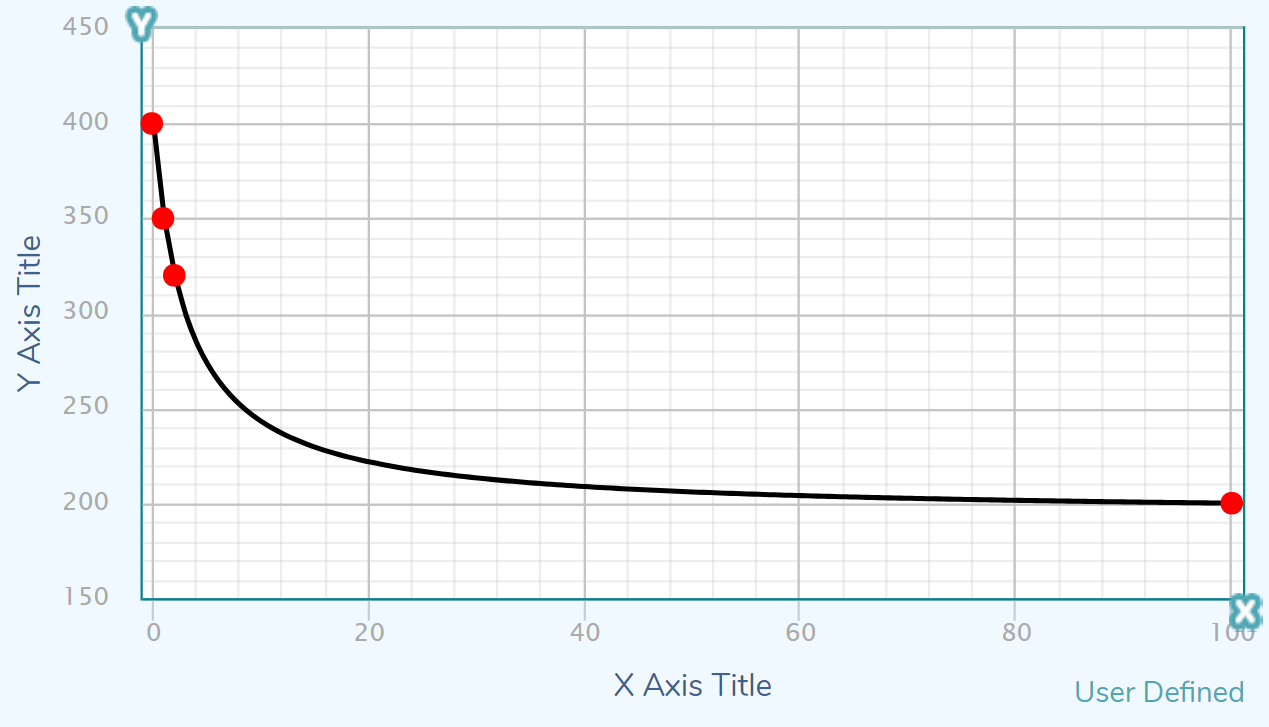
\includegraphics[width=0.48\textwidth, height=4cm]{curve-fit}
\\

The difficulty of sealing block for \textit{n} sealers will be calculated in the formula \eqref{eq:difficulty} as below

\begin{equation}\label{eq:difficulty}
    d(i) \equiv
    \begin{cases}
    	n	& \quad \text{if } sealer \text{ is in-turn}\\
	n - k_i & \quad \text{if } sealer \text{ is out-turn}
    \end{cases}
\end{equation}

${k_i}$ is the relative position of \textit{out-turn} sealer ${i^{th}}$ to the position of \textit{in-turn} sealer in the current sealing order list.

\section{Nexty Governance}\label{sec:governace}

This section will describe detail implementation of registration smart contract deployed at address \textbf{0x12345} using for consensus system.

\subsection{Terminology}

\begin{description}
\item[sealer] a participant in the Nexty consensus system. You can become one by depositing {\small DEPOSIT\_SIZE} {\small NTFs} into the Nexty mechanism.
\item[active sealer set] those sealer who are currently participating, and which the Nexty mechanism looks to seal blocks and other consensus objects.
\item[withdrawal period] number of epochs between a sealer exit and the sealer balance being withdraw-able.
\item[coinbase] the account address that sealer will use to sign when sealing block.
\item[registration contract] a smart contract for handling Nexty consensus mechanism.
\end{description}

\subsection{Constants}

\begin{center}
  \begin{tabular}{{l|l|l}}
    \hline
    Constant & Value & Unit \\
    \hline
    BLOCK\_TIME & ${2}$ & seconds \\
    EPOCH\_LENGTH & ${3,000}$ & blocks \\
    DEPOSIT\_SIZE & ${50,000}$ & {\small NTFs} \\
    WITHDRAWAL\_PERIOD & ${30,000}$ & blocks \\
    \hline
  \end{tabular}
\end{center}

\subsection{Sealer status codes}

\begin{description}
\item[PENDING\_ACTIVE = 0] Sealer deposited enough {\small NTFs} into registration contract successfully. 
\item[ACTIVE = 1] Sealer send request to become a sealer and added into activation sealer set successfully.
\item[PENDING\_WITHDRAW = 2] Sealer send request to exit from activation sealer set successfully. Sealer casted out of activation sealer set.
\item[WITHDRAWN = 3] Sealer already withdrawn their deposit {\small NTFs} successfully. They can only make withdrawal after withdrawal period.
\item[PENALIZED = 127] Sealer marked as penalized node (update by consensus or voting result via dapp) and cannot become active sealer and cannot withdraw balance neither.
\end{description}

\subsection{Nexty chain registration contract}
A registration contract is added to the Nexty chain to deposit {\small NTF} and activation sealer set management. It has some below basic functions:

\subsubsection{Sealer Operations}
\begin{description}
\item[Deposit] Transfer the {\small NTF} from token holder to registration contract. Sealer might have to approve contract to transfer an amount of {\small NTF} before calling this function.
\item[Join] To allow deposited {\small NTF} participate joining in as sealer. Participate already must deposit enough {\small NTF} via \textbf{Deposit} function. it takes \textbf{coinbase} as parameter.
\item[Exit] Request to exit out of activation sealer set.	
\item[Withdraw] To withdraw sealer’s {\small NTF} balance when they already exited and after \textbf{withdrawal period}.
\end{description}

\subsubsection{Sealer Record}
\begin{description}
\item[Coinbase address] sealer’s coinbase address to sign when sealing block
\item[Balance] the total amount of {\small NTF} that sealer has deposited
\item[Status] Sealer status code
\item[Requested Block Number] The block number at which sealer send request to exit out of activation sealer set.
\end{description}

\subsection{How to become a sealer}
\begin{enumerate}
\item A participant should deposit at least {\small DEPOSIT\_SIZE} {\small NTFs} into registration contract, a.k.a the network have maximum ~200 candidate nodes can become a sealer. Sealer status will be set to {\small PENDING\_ACTIVE}.
\item A participant need to set their \textbf{coinbase} to seal the block and receive reward on their equivalent {\small NTF} token holder address.
\item A participant call registration contract method to become sealer. Sealer status be updated to {\small ACTIVE}.
\item At next checkpoint of the epoch, sealer request be cast and the sealer be added into consensus \textbf{activation sealer set}.
\end{enumerate}

\subsection{How to exit from activation sealer and NTF withdrawal}
\begin{enumerate}
\item Sealer call registration contract method to request for exiting from activation sealer set and sealer status be updated to {\small PENDING\_WITHDRAW} but still in the activation sealer set on the current epoch.
\item At next checkpoint of the epoch, sealer exit request be cast and the sealer be removed out of \textbf{activation sealer set}. 
\item Sealer can call register contract method to withdrawn their deposited {\small NTF} after a withdrawal period. The sealer status be changed to {\small WITHDRAWN} after sealer withdraw the {\small NTFs} successfully.
\end{enumerate}

\subsection{Sealer authorization}
When a node starting with --${mine}$ option then they need to unlock the unique \textbf{coinbase} account setting in the activation sealer set. If the \textbf{coinbase} was not found in the current epoch \textbf{activation sealer set} then unauthorization error will be throw and it cannot start mining but they still can continue to sync block preparing for sealing later.

\subsection{Penalized}

At the checkpoint of each epoch, consensus will collect the data from the chain to find out any sealers that didn't seal any blocks 3 epochs in a row. Then to ensure the network healthy, those sealers will be removed out of the \textbf{activation sealer set} in the new epoch and mark sealer's status as {\small PENALIZED}. Because, offline sealers may due to the nature of unstable global network and dis-continue infrastructure service that out of control of the sealers. Then all {\small PENALIZED} sealers then can be unlock the slash after voting up by {\small NTY} community via a specific voting smart contract as well as dapp. 

\section{Block sealer reward calculation}

Reward will be added immediately into sealer’s account balance after sealing a block. The reward for a block is equal to the number of rewards per year divided by $\mathbf{15,768,000}$, the expected number of block within one year (initial configuration of block time is 2 seconds). The amount of rewards of each block sealing in a specific year is calculated in the following proportions:

\begin{center}
  \begin{tabular}{c | l | l}
    \hline
    Year &  \% of total supply & Reward/Blk\\ 
    \hline
    1 & 10.000 & 1,141\\ 
    2 & 5.000 & 627 \\ 
    3 & 2.500 & 329 \\ 
    4 & 1.250 & 169 \\ 
    5 & 0.625 & 85 \\
    6 & 0.500 & 69 \\
    ... & 0.500 & ... \\
    ... & 0.500 & ... \\ 
    n & 0.500 & ... \\
    \hline
  \end{tabular}
\end{center}

\section{Anti-SPAM}\label{sec:spam}

\subsection{Most Frequency Use}\label{sec:mfu}

In Nexty blockchain, we allow end user to perform transaction with zero fee. Therefore, we introduce a mechanism to priority transactions base on some other factors other than using only the \textbf{gasprice}. The first factor is similar to stamina, each account will have a \textbf{most frequency use} state. whenever, transaction from account to include in the block then the \textbf{most frequency use}, ${\Delta_{new}}$, will be update as following formula.

\begin{equation}
	{\Delta_{new}}  = {\Delta_{old}} + max(1, \frac{(block - {\Delta_{old}}) * GasUsed}{3 * 21000})
\end{equation}

\begin{description}
\item[block] is the block number that transaction was include.
\item[GasUsed] gas used by the transaction
\end{description}

Ideally, the higher \textbf{most frequency use} value, the less priority of the account's transaction in the transaction pool. And each time an account perform the transaction, \textbf{most frequency use} value of that account will be increase; as a result, the next transaction of the same account will be less priority. And to avoid spam by new account, the \textbf{most frequency use} of a new account will be the block number of the account's first transaction.

\subsection{Transaction Parity}\label{sec:parity}

Along with  \textbf{most frequency use} above, we introduce a new factor to decide the priority of the transaction called \textbf{parity} and will be calculated as below

\begin{equation}\label{eq:parity}
{\rho_t} = {\Delta_{act}} + \frac{TxGasLimit}{21000} - \frac{TxGasPrice}{ParityLimit}
\end{equation}

\begin{description}
\item[${\Delta_{act}}$] \textbf{most frequency use} value of the account when perform transaction
\item[TxGasLimit] transaction gas limit, the higher gas limit transaction, the less priority
\item[TxGasPrice] transaction gas price, can be input arbitrarily by user. User can put higher gas price if they want to make transaction be confirmed faster.
\item[ParityLimit] parity limit be configured by miner, the higher parity limit, the less transaction gas price effect into the overall parity value, ${\rho_t}$
\end{description}

Overall, a transaction was include in the miner's txpool with priority base on the value of transaction parity calculated in formula \eqref{eq:parity} then even though Nexty allow user to send tnx with zero fee but sealer's pool can arbitrarily setting parameters to utilize the sealer's resource for anti spamming transaction and ensure normal user's transaction to be proceed without delay.

\subsection{Transaction Proof of Work}
In the near future, when the Nexty chain will be fulfilled or be spammed by unmeaning transactions, we will introduce a mechanism to avoid those kind of problem by enforcing user to send a proof of mini work along with the transaction, the transaction with valid proof will be sealed in the block with highest priority. To make a better user experience and adoption, we will develop this feature in user wallet; when the transaction confirmation is too slow, wallet will allow user to take action to do transaction proof of work on their wallet before sending transaction.

\bibliographystyle{plainnat}
\bibliography{Biblio}

\end{multicols}
\end{document}